\section{Ergebnis}

Screenshots vom Ergebnis zeigen
ggf. Unterschiede zum Mockup + Anforderungen

\subsection{Admin}

\begin{figure}[tbh]
\centering
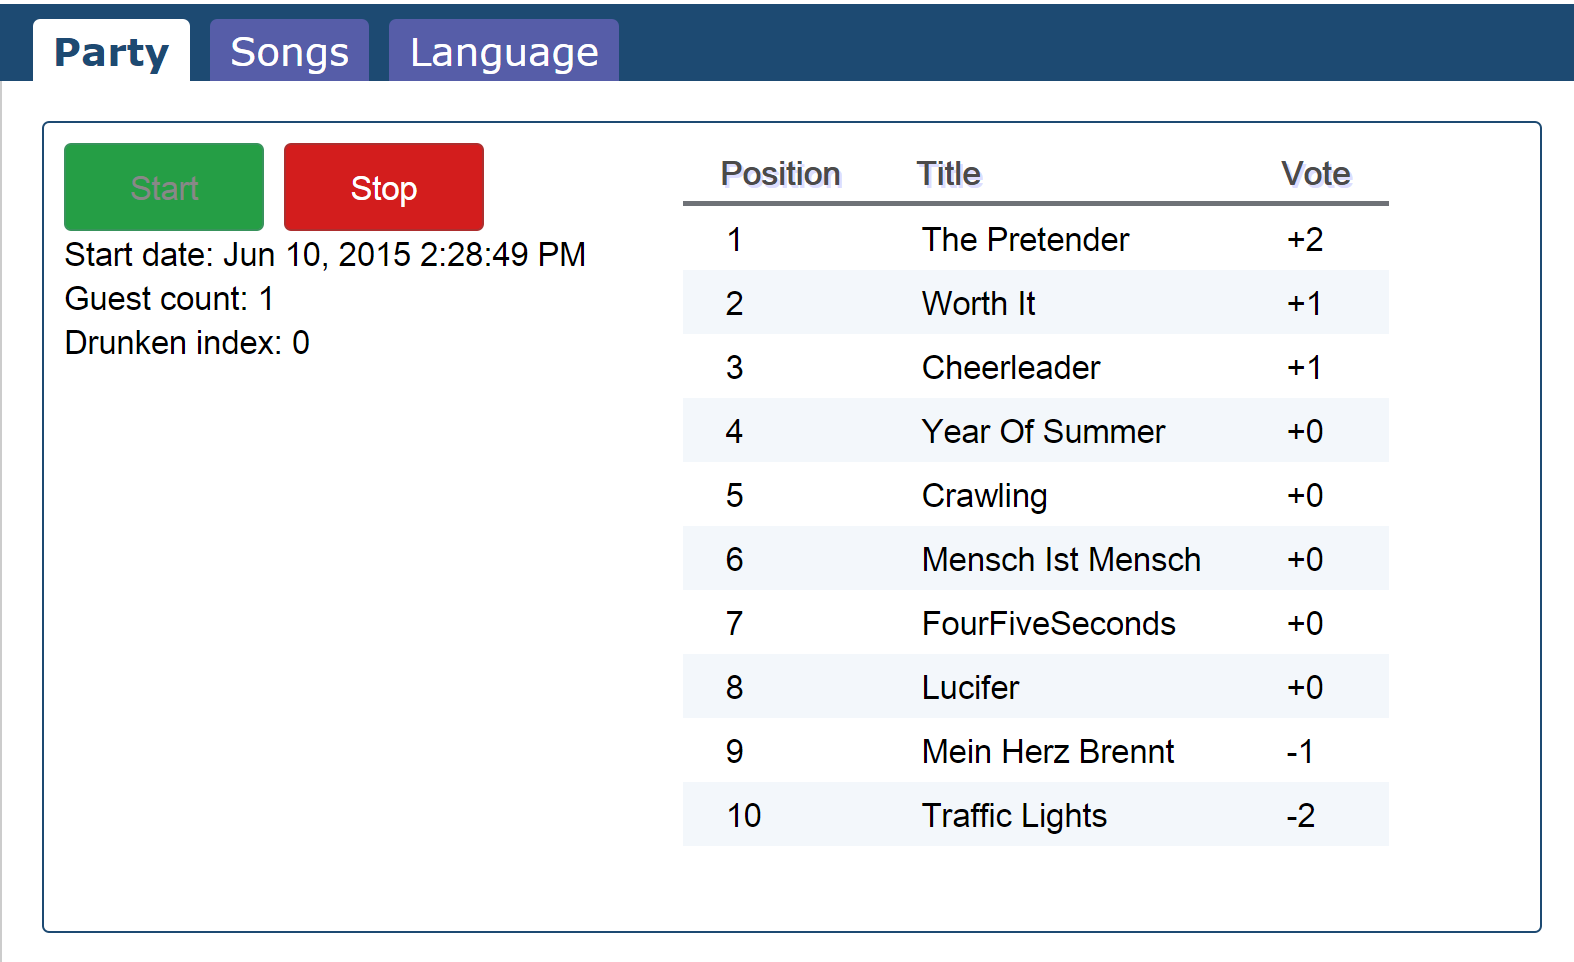
\includegraphics[width=1.0\linewidth]{Bilder/Screenshot-Admin-Party}
\caption{Screenshot der Admin-Oberfläche: Party verwalten}
\label{fig:Screenshot-Admin-Party}
\end{figure}

\begin{figure}[tbh]
\centering
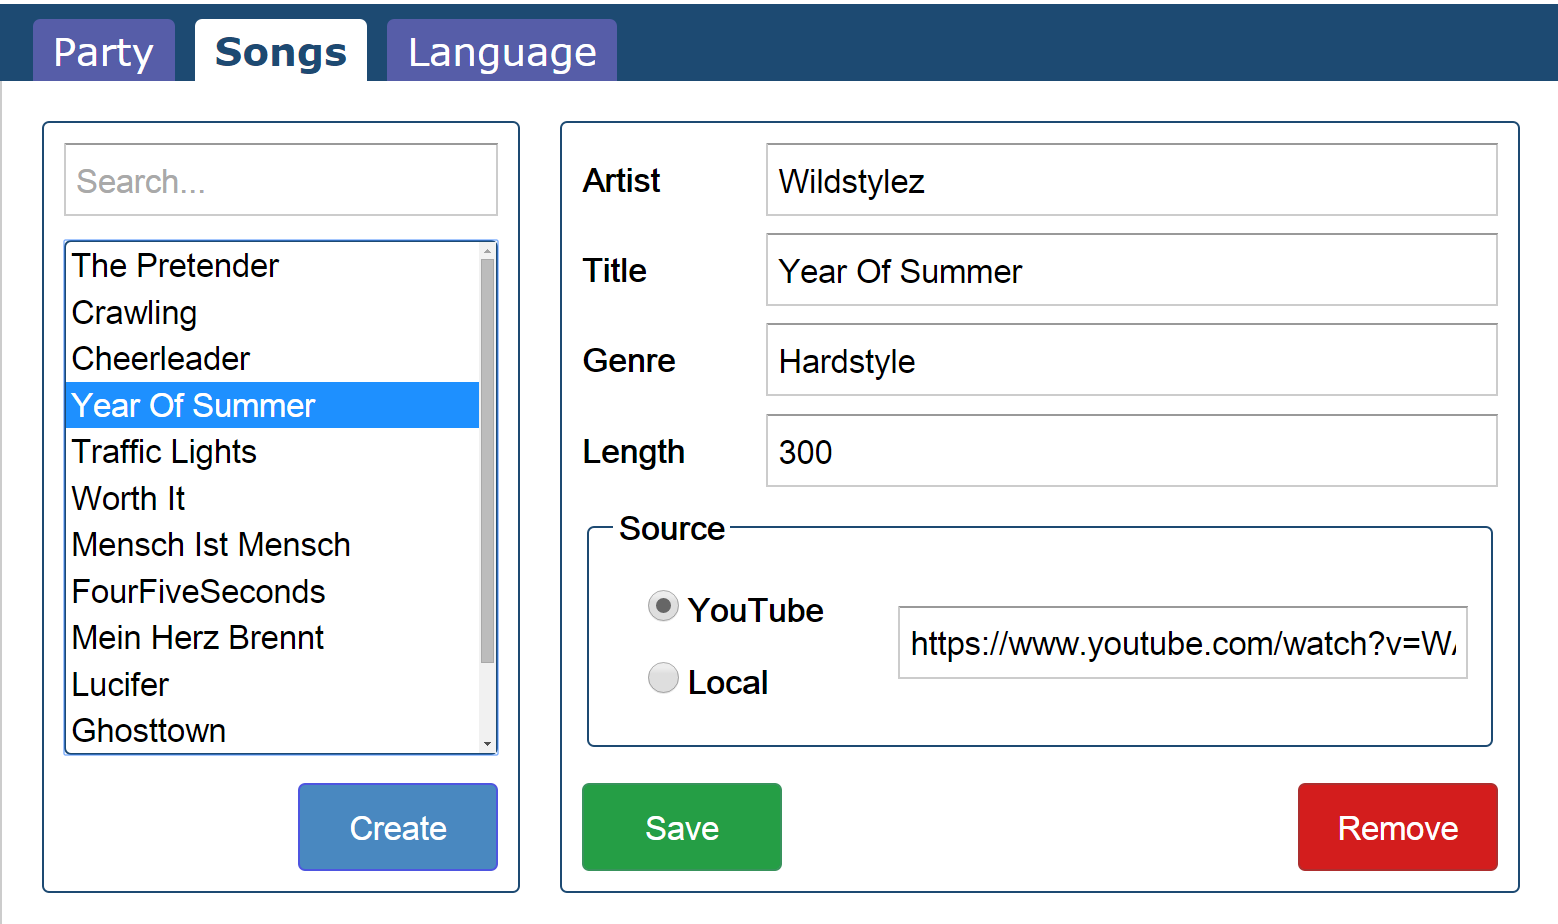
\includegraphics[width=1.0\linewidth]{Bilder/Screenshot-Admin-Songs}
\caption{Screenshot der Admin-Oberfläche: Songs verwalten}
\label{fig:Screenshot-Admin-Songs}
\end{figure}

\begin{figure}[tbh]
\centering
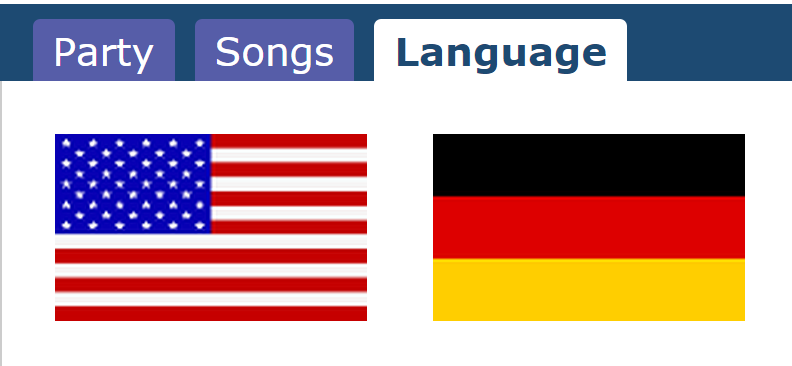
\includegraphics[width=0.7\linewidth]{Bilder/Screenshot-Admin-Language}
\caption{Screenshot der Admin-Oberfläche: Sprachauswahl}
\label{fig:Screenshot-Admin-Language}
\end{figure}


\subsection{Vote-App}

\begin{figure}[tbh]
\centering
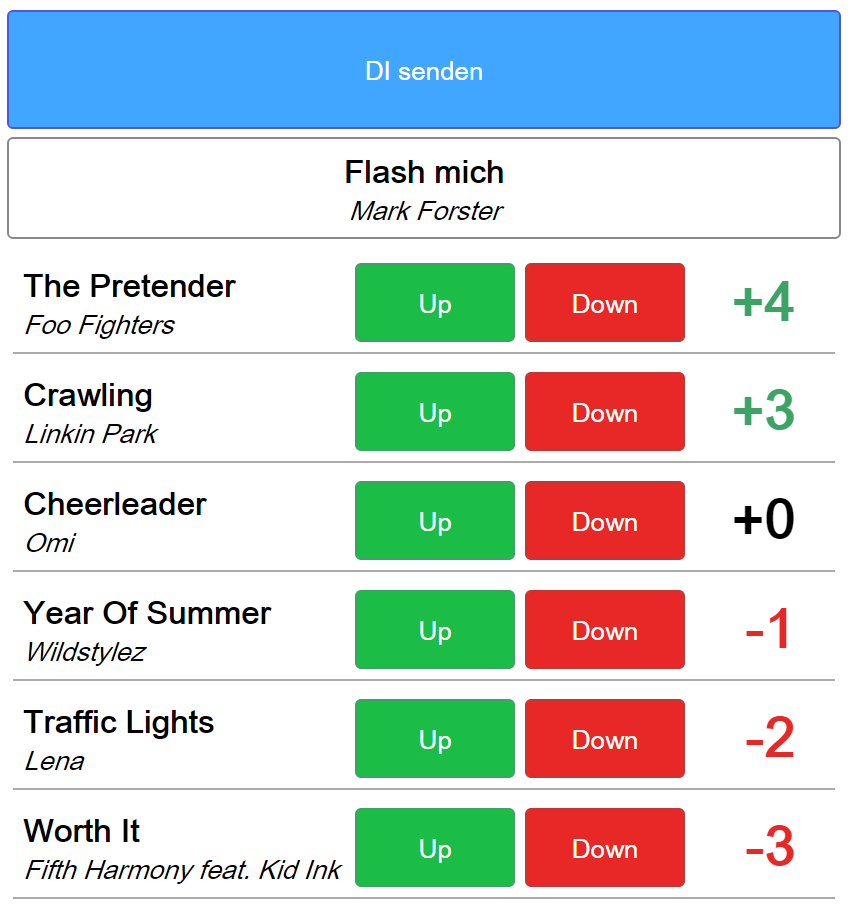
\includegraphics[width=0.7\linewidth]{Bilder/Screenshot-Vote-App}
\caption{Screenshot der Vote-App}
\label{fig:Screenshot-Vote-App}
\end{figure}


Daniel??